\documentclass[12pt]{report}
\usepackage[utf8]{inputenc}
\usepackage[russian]{babel}
%\usepackage[14pt]{extsizes}
\usepackage{listings}

% Для листинга кода:
\lstset{ %
language=python,                 % выбор языка для подсветки (здесь это С)
basicstyle=\small\sffamily, % размер и начертание шрифта для подсветки кода
numbers=left,               % где поставить нумерацию строк (слева\справа)
numberstyle=\tiny,           % размер шрифта для номеров строк
stepnumber=1,                   % размер шага между двумя номерами строк
numbersep=5pt,                % как далеко отстоят номера строк от подсвечиваемого кода
showspaces=false,            % показывать или нет пробелы специальными отступами
showstringspaces=false,      % показывать или нет пробелы в строках
showtabs=false,             % показывать или нет табуляцию в строках
frame=single,              % рисовать рамку вокруг кода
tabsize=2,                 % размер табуляции по умолчанию равен 2 пробелам
captionpos=t,              % позиция заголовка вверху [t] или внизу [b] 
breaklines=true,           % автоматически переносить строки (да\нет)
breakatwhitespace=false, % переносить строки только если есть пробел
escapeinside={\#*}{*)}   % если нужно добавить комментарии в коде
}

% Для измененных титулов глав:
\usepackage{titlesec, blindtext, color} % подключаем нужные пакеты
\definecolor{gray75}{gray}{0.75} % определяем цвет
\newcommand{\hsp}{\hspace{20pt}} % длина линии в 20pt
% titleformat определяет стиль
\titleformat{\chapter}[hang]{\Huge\bfseries}{\thechapter\hsp\textcolor{gray75}{|}\hsp}{0pt}{\Huge\bfseries}


% plot
\usepackage{pgfplots}
\usepackage{filecontents}
\usetikzlibrary{datavisualization}
\usetikzlibrary{datavisualization.formats.functions}

\begin{document}
 
%\def\chaptername{} % убирает "Глава"
\begin{titlepage}
	\centering
	{\scshape\LARGE МГТУ им. Баумана \par}
	\vspace{3cm}
	{\scshape\Large Лабораторная работа №5\par}
	\vspace{0.5cm}	
	{\scshape\Large По курсу: "Операционные системы"\par}
	\vspace{1.5cm}
	{\huge\bfseries Буферизованный и не буферизованный ввод-вывод\par}
	\vspace{2cm}
	\Large Работу выполнил: студент группы ИУ7-63Б Наместник Анастасия\par
	\vspace{0.5cm}
	\LargeПреподаватели:  Рязанова Н. Ю.\par

	\vfill
	\large \textit {Москва, 2021} \par
\end{titlepage}

%\tableofcontents

\newpage
	
\section{Задание}
%\addcontentsline{toc}{chapter}{Введение}
В лабораторной работе анализируется результат выполнения трех программ. Программы демонстрируют открытие одного и того же файла несколько раз. Реализация открытия файла в одной программе несколько раз выбрана для простоты. Такая ситуация возможна в системе, когда один и тот же файл несколько раз открывают разные процессы. Но для получения ситуаций аналогичных тем, которые демонстрируют приведенные программы надо было бы синхронизировать работу процессов. При выполнении асинхронных процессов такая ситуация вероятна и ее надо учитывать, чтобы избежать потери данных или получения неверного результата при выводе в файл.	
		
\section{Программа 1}

Код программы:

\begin{lstlisting}[language=C]
//testCIO.c
#include <stdio.h>
#include <fcntl.h>

/*
On my machine, a buffer size of 20 bytes
translated into a 12-character buffer.
Apparently 8 bytes were used up by the
stdio library for bookkeeping.
 */

int main()
{
  // have kernel open connection to file alphabet.txt
  int fd = open("alphabet.txt",O_RDONLY);

  // create two a C I/O buffered streams using the above connection
  FILE *fs1 = fdopen(fd,"r");
  char buff1[20];
  setvbuf(fs1,buff1,_IOFBF,20);

  FILE *fs2 = fdopen(fd,"r");
  char buff2[20];
  setvbuf(fs2,buff2,_IOFBF,20);
  
  // read a char & write it alternatingly from fs1 and fs2
  int flag1 = 1, flag2 = 2;
  while(flag1 == 1 || flag2 == 1)
  {
    char c;
    flag1 = fscanf(fs1,"%c",&c);
    if (flag1 == 1)
    {
        fprintf(stdout,"%c",c);
    }
    
    flag2 = fscanf(fs2,"%c",&c);
    if (flag2 == 1)
    {
        fprintf(stdout,"%c",c);
    }
  }
  return 0;
}
\end{lstlisting}

Программа использует файл \textbf{alphabet.txt}, содержащий символы: Abcdefghijklmnopqrstuvwxyz.

В результате выполнения программы в стандартный поток вывода stdout запишется следующая последовательность символов:  Aubvcwdxeyfzghijklmnopqrst.

\section{Анализ первой программы}

В стандартную библиотеке C stdio.h включен заголовочный файл, полный путь которого \textit{glibc/libio/bits/types/FILE.h}, содержащий объявление структуры FILE:

\begin{lstlisting}[language=C]
#ifndef __FILE_defined
#define __FILE_defined 1
	
struct _IO_FILE;
	
/* The opaque type of streams.  This is the definition used elsewhere.  */
typedef struct _IO_FILE FILE;
	
#endif	
\end{lstlisting}
описание которой содержится в файле \textit{glibc/libio/bits/types/struct\_FILE.h}:
\begin{lstlisting}[language=C]
struct _IO_FILE
{
  int _flags;                /* High-order word is _IO_MAGIC; rest is flags. */
 
  /* The following pointers correspond to the C++ streambuf protocol. */
  char *_IO_read_ptr;        /* Current read pointer */
  char *_IO_read_end;        /* End of get area. */
  char *_IO_read_base;        /* Start of putback+get area. */
  char *_IO_write_base;        /* Start of put area. */
  char *_IO_write_ptr;        /* Current put pointer. */
  char *_IO_write_end;        /* End of put area. */
  char *_IO_buf_base;        /* Start of reserve area. */
  char *_IO_buf_end;        /* End of reserve area. */
 
  /* The following fields are used to support backing up and undo. */
  char *_IO_save_base; /* Pointer to start of non-current get area. */
  char *_IO_backup_base;  /* Pointer to first valid character of backup area */
  char *_IO_save_end; /* Pointer to end of non-current get area. */
 
  struct _IO_marker *_markers;
 
  struct _IO_FILE *_chain;
 
  int _fileno;
  int _flags2;
  __off_t _old_offset; /* This used to be _offset but it's too small.  */
 
  /* 1+column number of pbase(); 0 is unknown. */
  unsigned short _cur_column;
  signed char _vtable_offset;
  char _shortbuf[1];
 
  _IO_lock_t *_lock;
#ifdef _IO_USE_OLD_IO_FILE
};	
\end{lstlisting}

Структура FILE - сущность языка C и его стандартной библиотеки stdio.h. При работе со структурой FILE автоматически создается буфер, и программист работает с более высокоуровневой абстракцией. Объект типа FILE содержит информацию о файле и  обращается к соответствующему файловому дескриптору Unix. 

Размер буфера по дефолту в stdio.h:
\begin{lstlisting}[language=C]
/* Default buffer size.  */
#define BUFSIZ 8192	
\end{lstlisting}

Связь структур представлена на рисунке 0.1

\begin{center}
		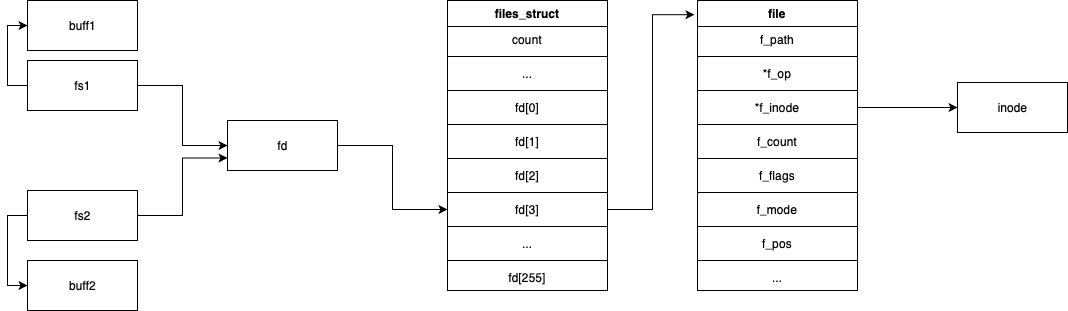
\includegraphics[scale=0.45]{pics/proc1.png}
		
			Рис 0.1: Связь структур для первой программы
\end{center}

В функции main() вызывается функция open(), вызывающая, в свою очередь, системный вызов (system call) open() для чтения файла alphabet.txt,  содержащего последовательность символов латинского алфавита: Abcdefghijklmnopqrstuvwxyz. Возвращаемое значение - целое неотрицательное число (int) - индекс в массиве fd\_array[NP\_OPEN\_DEFAULT] структур типа file, определенном в таблице открытых файлов процесса - \textit{struct files\_struct}. Полученное число является \textbf{файловым дескриптором} файла alphabet.txt.

Функция fdopen() может использоваться для инициализации структуры FILE файловым дескриптором.
С помощью функции fd\_open(), принимающей fd создаются два указателя fs1 и fs2 типа struct FILE, ссылающиеся на структуру типа file в массиве fd\_array[NP\_OPEN\_DEFAULT] с индексом, равным fd. 

Иными словами, fs1 и fs2 ссылаются на файловый дескриптор, полученный с помощью open(), так как fd\_open() передается файловый дескриптор, созданный с помощью open().

С помощью функции setvbuf() для fs1 и fs2 создается два буфера на 20 байт, тип буферизации - полная буферизация. Содержимое буферов buff1 и buff2 после вызова fscanf() для fs1 и затем для fs2 представлено на рисунке 0.2.

\begin{center}
		
\includegraphics[scale=0.6]{pics/buff.png}
		
			Рис 0.2: buff1 и buff2 после вызова fscanf()
\end{center}

Такой результат объясняется тем, что сначала полностью заполняется buff1 первыми 20 символами - Abcdefghijklmnopqrst, а затем остаток данных файла alphabet.txt записывается в buff2 - uvwxyz. Это происходит благодаря тому, что указатель f\_pos структуры file, описывающей файл, имеющий дескриптор fd, увеличивается на 20 после выполнения первой операции чтения fscanf(fs1,"\%c",\&c). Так как обе структуры FILE fs1 и fs2 ссылаются на одну и ту же запись в таблице открытых файлов процесса, при вызове fscanf(fs2,"\%c",\&c) произойдет обращение к тому же указателю f\_pos.

Далее в цикле содержимое буферов buff1 и buff2 попеременно выводится в стандартный поток вывода stdout, что можно видеть на рисунке 0.3.

\begin{center}
		
\includegraphics[scale=0.6]{pics/Res1.png}
		
			Рис 0.3: Результат работы первой программы
\end{center}

\section{Программа 2 (2 процесса)}

Код программы (главный процесс):

\begin{lstlisting}[language=C]
//testKernelIO.c
#include <fcntl.h>

int main()
{
    char c;
  // have kernel open two connection to file alphabet.txt
    int fd1 = open("alphabet.txt",O_RDONLY);
    int fd2 = open("alphabet.txt",O_RDONLY);
  // read a char & write it alternatingly from connections fs1 & fd2
    int flag = 1;
    
    while(flag)
    {
        if (read(fd1,&c,1) == 1)
            write(1,&c,1);
        else
            flag = 0;
    
        if (read(fd2,&c,1) == 1)
            write(1,&c,1);
        else
            flag = 0;
  }
    return 0;
}
\end{lstlisting}

Код программы (процесс-предок и процесс-потомок):

\begin{lstlisting}[language=C]
//testKernelIO.c
#include <stdio.h>
#include <fcntl.h>
#include <unistd.h>

int main()
{
   char c;
  // have kernel open two connection to file alphabet.txt
  int fd1;
  int fd2 = open("alphabet.txt",O_RDONLY);
  // read a char & write it alternatingly from connections fs1 & fd2
  int flag = 1;
  int pid;
  
  if ((pid = fork()) == -1)
  {
    perror("fork Error\n");
    return 0;
  }
    
  if (pid == 0)
      fd1 = open("alphabet.txt",O_RDONLY);

  while(flag)
  {
    if (pid == 0) //child process
    {
      if (read(fd1,&c,1) == 1)  //-1 if fails to read
        write(1,&c,1);
      else 
        flag = 0;
      printf("Child process = %d\n", getpid());
    }

    else
    {
      if (read(fd2,&c,1) == 1)
        write(1,&c,1);
      else
        flag = 0;
      printf("Parent process = %d\n", getpid());
    }
  }
  
  return 0;
}
\end{lstlisting}

\section{Анализ второй программы (2 процесса)}

\subsection{Главный процесс}

Файл alphabet.txt открывается 2 раза с помощью 2-х вызовов open() с режимом доступа на чтение - O\_RDONLY. Следовательно, в таблице открытых файлов процесса будет находиться 2 дескриптора, с которыми будут связаны две записи в системной таблице открытых файлов, указатель *f\_inode которых будет указывать на один inode, так как дескрипторы fd1 и fd2 описывают один файл. 

Связь структур представлена на рисунке 0.4.

\begin{center}
		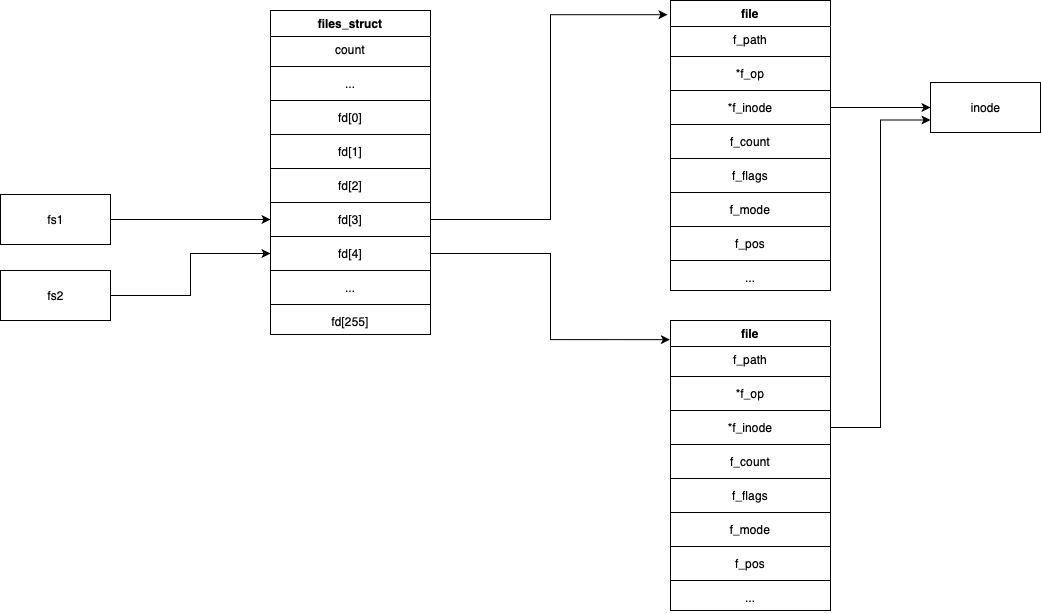
\includegraphics[scale=0.45]{pics/proc2.png}
		
			Рис 0.4: Связь структур для второй программы (главный процесс)
\end{center}

Результат работы второй программы без использования процесса-потомка представлен на рисунке 0.5.

\begin{center}
		
\includegraphics[scale=0.6]{pics/Res2.png}
		
			Рис 0.5: Результат работы второй программы (главный процесс)
\end{center}

Символы записываются в стандартный поток вывода stdout попеременно, дублируясь, так как для дескрипторов fd1 и fd2 имеется две разных структуры file, и, соответственно, указатель позиции на чтение/запись в файле *f\_pos будет независимым для них.

\subsection{Процесс-предок и процесс-потомок}

Чтобы создать процесс-потомок, используется вызов fork(), после которого процесс-предок считывает из одного открытого файла (с использованием fd1), а процесс-потомок - из другого открытого файла (с использованием fd2). При этом дескриптор fd2 был создан процессом-потомком, благодаря чему создается еще одна структура struct files\_struct - таблица открытых файлов процесса-потомка.

Связь структур для процесса-предка и процесса-потомка представлена на рисунке 0.6.

\begin{center}
		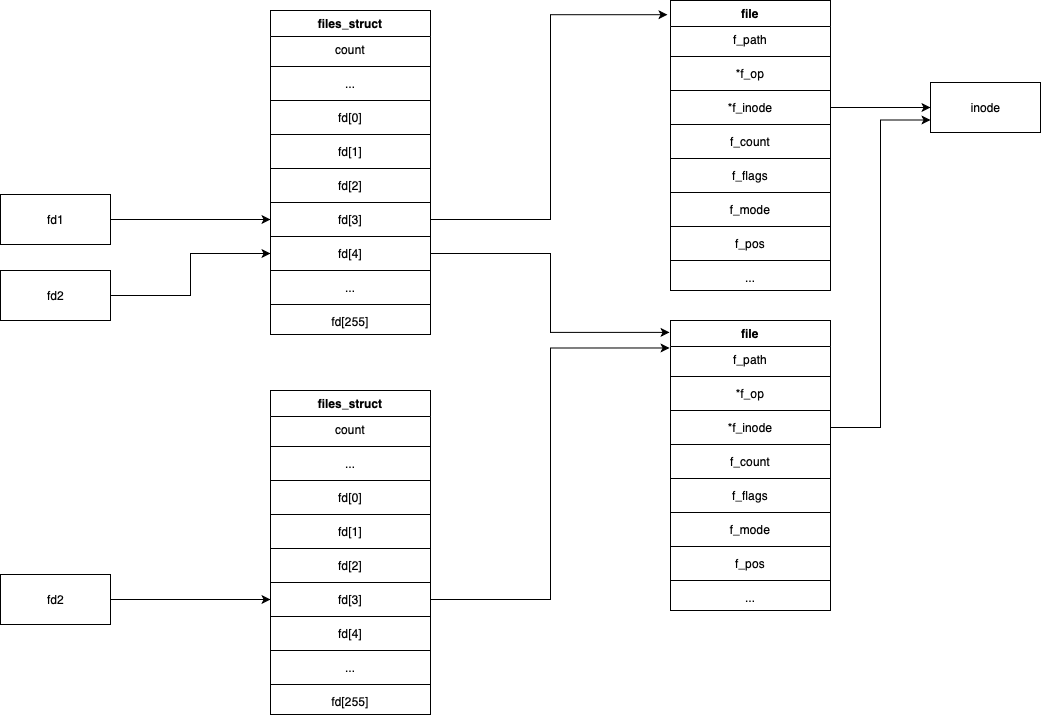
\includegraphics[scale=0.45]{pics/proc2_fork_2.0.png}
		
			Рис 0.6: Связь структур для второй программы (процесс-предок и процесс-потомок)
\end{center}

Результат работы второй программы с использованием процесса-потомка представлен на рисунке 0.7.

\begin{center}
		
\includegraphics[scale=0.5]{pics/Res2_4.png}
		
			Рис 0.7: Результат работы второй программы (процесс-предок и процесс-потомок)
\end{center}

На рисунках 08-0.10 представлен результат программы с более подробным анализом вывода за счет вывода на экран идентификаторов процессов.

\begin{center}
		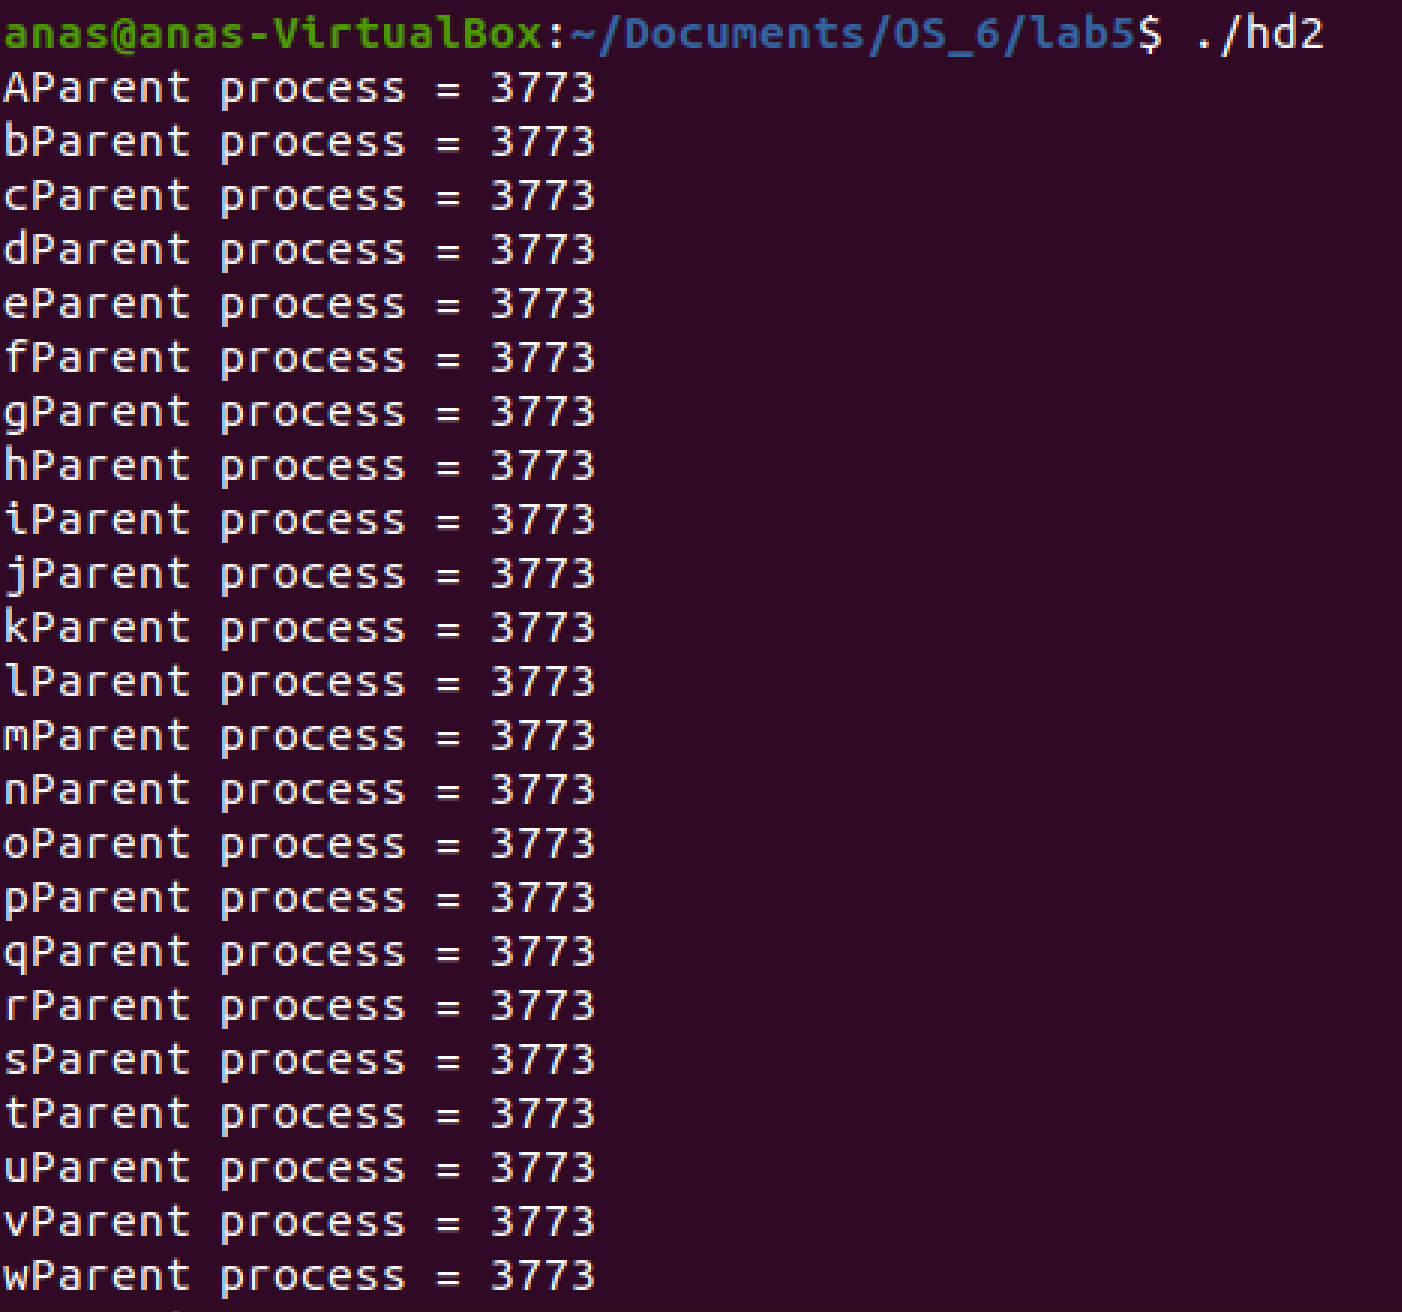
\includegraphics[scale=0.6]{pics/Res2_1.png}
		
			Рис 0.8: Анализ вывода с 2-умя процессами (1 часть)
\end{center}

\begin{center}
		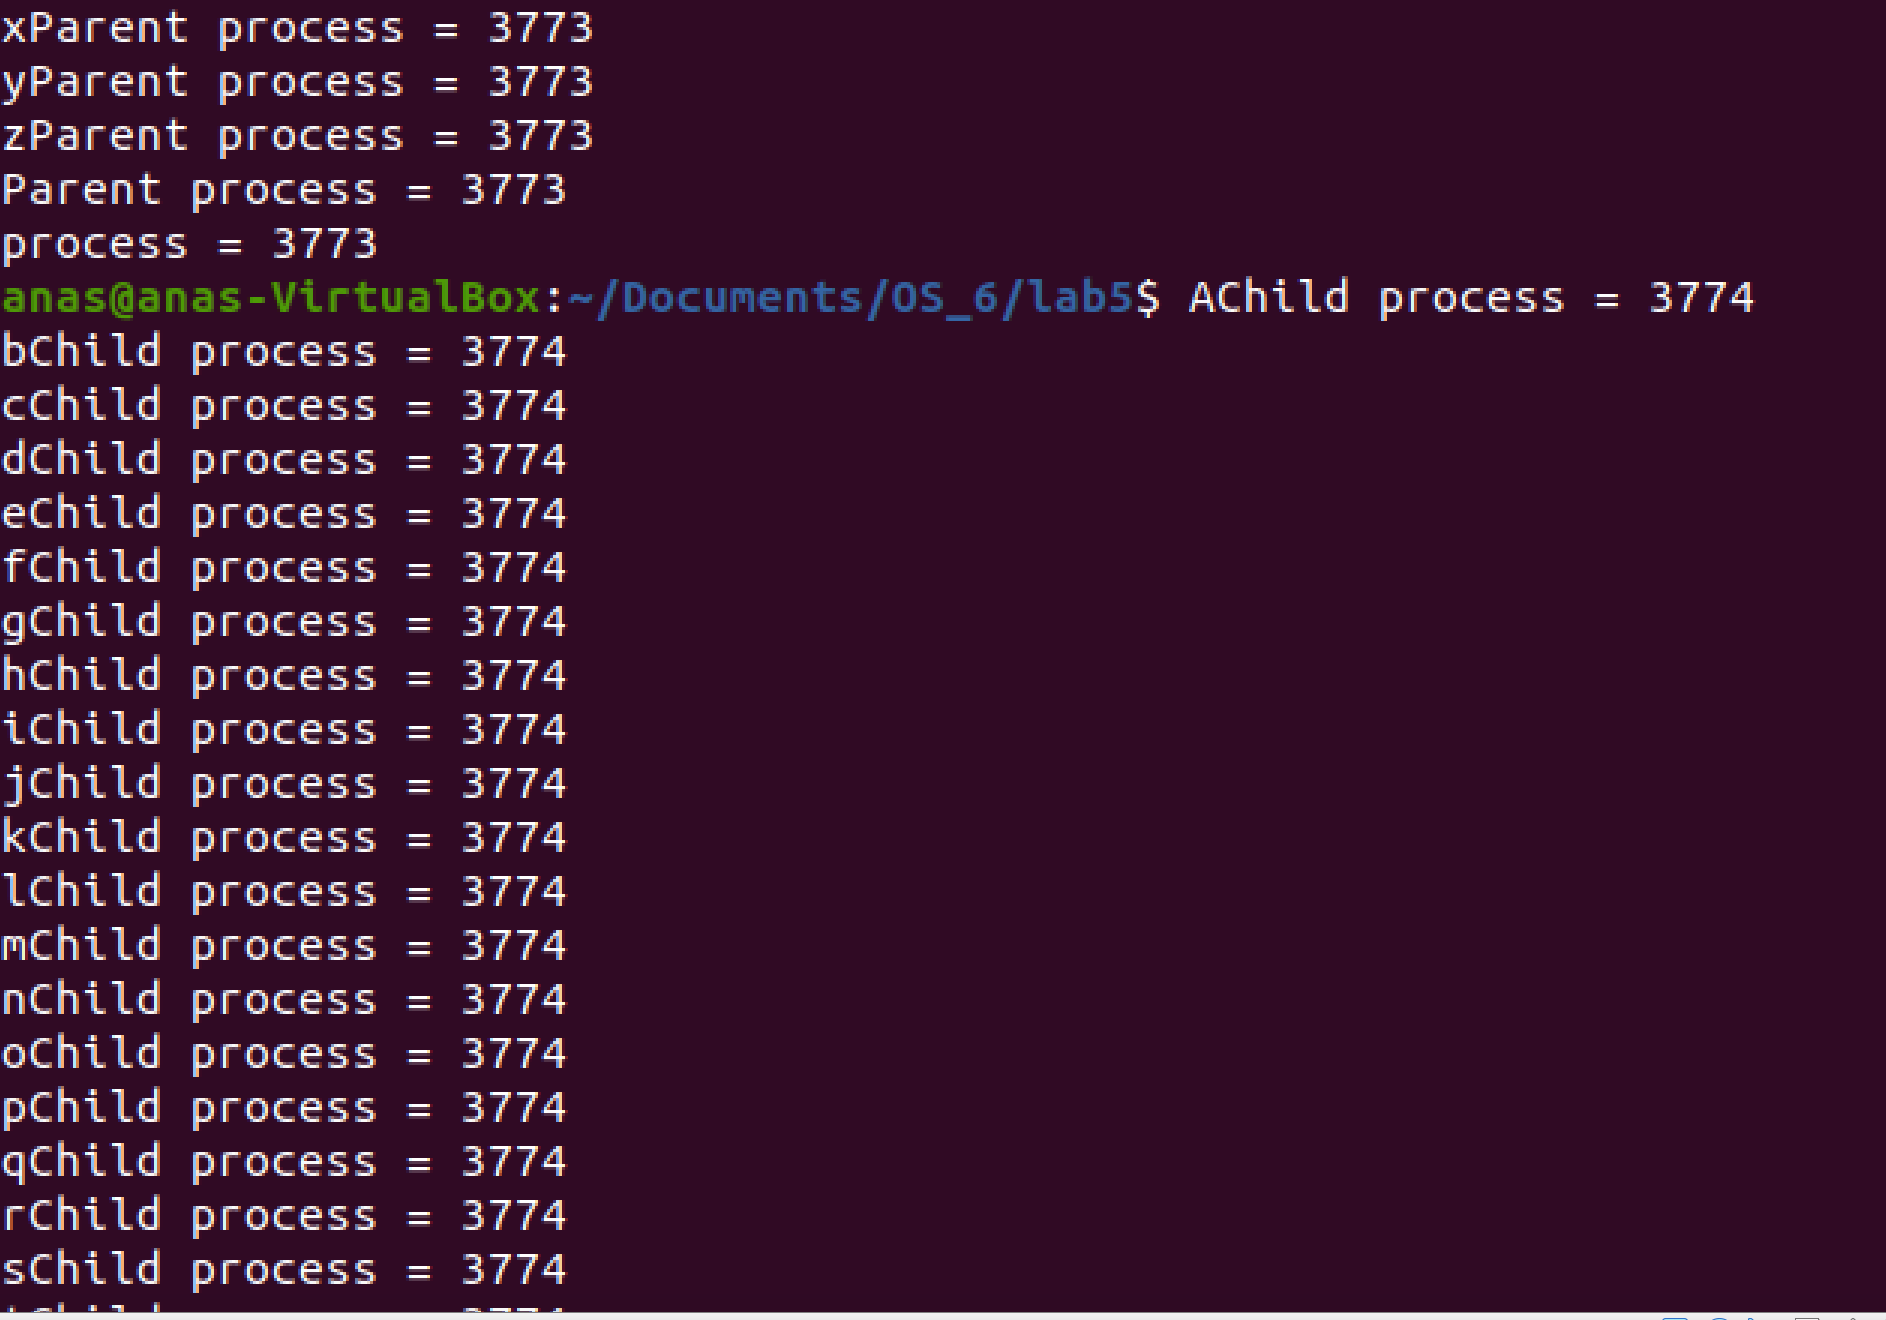
\includegraphics[scale=0.47]{pics/Res2_2.png}
		
			Рис 0.9: Анализ вывода с 2-умя процессами (2 часть)
\end{center}

\begin{center}
		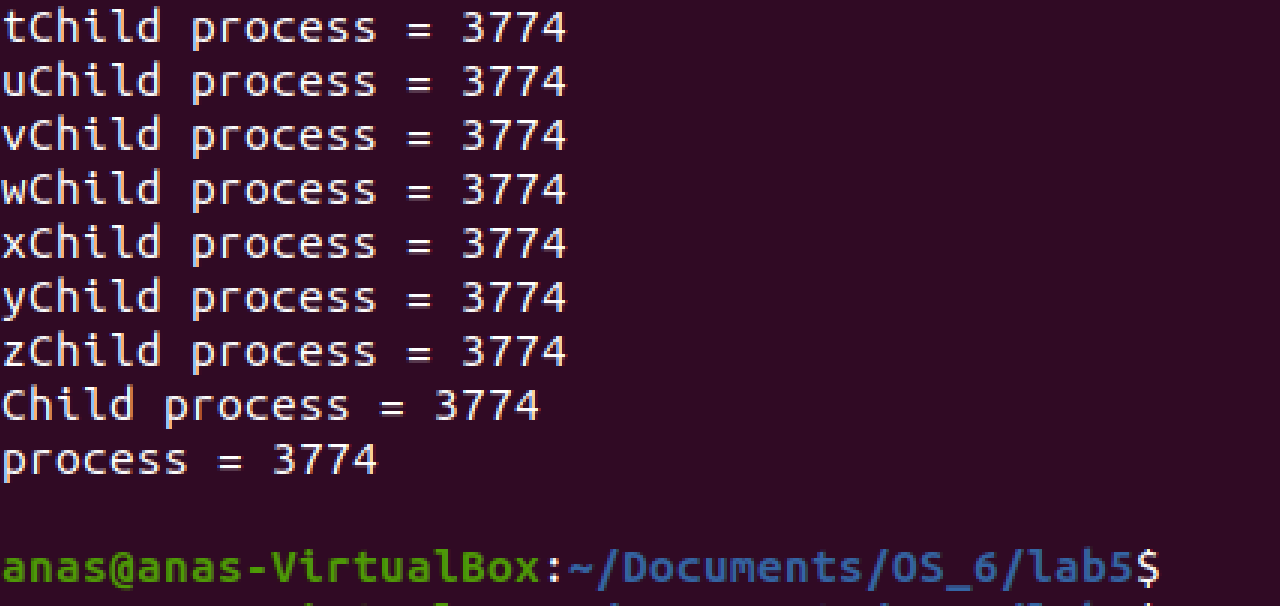
\includegraphics[scale=0.6]{pics/Res2_3.png}
		
			Рис 0.10: Анализ вывода с 2-умя процессами (3 часть)
\end{center}

\section{Программа 2 (2 потока)}

Код программы:

\begin{lstlisting}[language=C]
//testKernelIO.c
#include <stdio.h>
#include <pthread.h>
#include <fcntl.h>
#include <unistd.h> //System calls
#include <stdlib.h>
#define ERROR_CREATE_THREAD -11
#define ERROR_JOIN_THREAD   -12

typedef struct file_descr
{
  int fd;
} file_descr_t;

void *read_from_file(void *args)
{
  file_descr_t *file_descriptor = (file_descr_t*) args;
  char c;

  while(read(file_descriptor->fd, &c, 1) == 1)
    write(1, &c, 1);
  
  write(1, " ", 1);
}

int main()
{
  char c;
  int status, status_addr;
  // have kernel open two connection to file alphabet.txt
  int fd1 = open("alphabet.txt",O_RDONLY);
  int fd2 = open("alphabet.txt",O_RDONLY);

  pthread_t thread;
 
  // read a char & write it alternatingly from connections fs1 & fd2
  status = pthread_create(&thread, NULL, read_from_file, &fd1);
  if (status != 0)
  { 
    printf("Error: couldn't create a thread. Status = %d\n", status);
    exit(ERROR_CREATE_THREAD);
  }

  read_from_file(&fd2);
   
  status = pthread_join(thread, (void**)&status_addr);
  if (status != 0) 
  {
        printf("Error: couldn't join thread. Status = %d\n", status);
        exit(ERROR_JOIN_THREAD);
    }
  
  return 0;
}

\end{lstlisting}

\section{Анализ второй программы (2 потока)}

С помощью функции \textit{pthread\_create()}, объявленной в заголовочном файле pthread.h, создается поток \textbf{thread}, который будет читать из одного открытого файла, в то время как главный поток читает из другого открытого файла. Таким образом, реализовано параллельное чтение из двух открытых файлов, имеющих дескрипторы fd1 и fd2.

Результат работы второй программы с использованием 2-х потоков представлен на рисунке 0.11.

\begin{center}
		
\includegraphics[scale=0.42]{pics/Res2_threads.png}
		
			Рис 0.11: Результат работы второй программы (2 потока)
\end{center}

Связь структур в случае с использованием 2-ух потоков представлена на рисунке 0.4.

\section{Программа 3}

Код программы:

\begin{lstlisting}[language=C]
#include <stdio.h>
#include <fcntl.h>
#include <pthread.h>
#include <sys/stat.h>
#include <time.h>
#include <stdlib.h> //exit
#define ALPHABET "Abcdefghijklmnopqrstuvwxyz"
#define ALPHABET_SIZE 26
#define FILENAME "proc3_alphabet.txt"
#define ERROR_CREATE_THREAD -11
#define ERROR_JOIN_THREAD   -12

void print_stat(char *fd, char *operation, struct stat statbuf)
{
	printf("%s_%s:\ninode: %d\nsize: %d\nI/O_block_size: %d\nLast modification of file data: %s\n", 
		fd, operation, (int)statbuf.st_ino, 
		(int)statbuf.st_size, (int)statbuf.st_blksize, ctime(&statbuf.st_mtime));

}

typedef struct file_descr
{
	FILE *fd;
} file_descr_t;

void *read_from_file(void *args)
{
	file_descr_t *file_descriptor = (file_descr_t*) args;
	char c;

	for (int i = 0; i < ALPHABET_SIZE; i+=2)	
		fprintf(file_descriptor->fd, "%c", ALPHABET[i]); //acegikmoqsuwy
}

int main()
{
	struct stat statbuf;
	pthread_t thread;
	int status, status_addr;

	FILE *fd1 = fopen(FILENAME, "w");
	stat(FILENAME, &statbuf);
	print_stat("fd1", "fopen", statbuf);

	FILE *fd2 = fopen(FILENAME, "w");
	stat(FILENAME, &statbuf);
	print_stat("fd2", "fopen", statbuf);

	status = pthread_create(&thread, NULL, read_from_file, &fd1);
  	if (status != 0)
  	{ 
    	printf("Error: couldn't create a thread. Status = %d\n", status);
    	exit(ERROR_CREATE_THREAD);
  	}	

	for (int i = 1; i < ALPHABET_SIZE; i+=2)	
		fprintf(fd2, "%c", ALPHABET[i]);

	status = pthread_join(thread, (void**)&status_addr);
  	if (status != 0) 
  	{
        printf("Error: couldn't join thread. Status = %d\n", status);
        exit(ERROR_JOIN_THREAD);
    }

	fclose(fd1);
	stat(FILENAME, &statbuf);
	print_stat("fd1", "fclose", statbuf);
	

	fclose(fd2);
	stat(FILENAME, &statbuf);
	print_stat("fd2", "fclose", statbuf);

	return 0;
}
\end{lstlisting}

\section{Анализ третьей программы}

Один и то же файл открывается 2 раза на запись. Для этого с помощью функции \textit{fopen()} объявляются 2 указателя на структуру типа FILE - fd1 и fd2. В обоих случаях функциях fopen() принимает имя файла - \textbf{"proc3\_alphabet.txt"} и режим доступа к файлу - \textbf{"w"}. Затем в цикле с помощью функции \textit{fprintf()} в файл записываются символы латинского алфавита, при этом созданные файловые дескрипторы используются попеременно - один за другим, что реализовано с помощью создания потока. Один поток читает из одного открытого файла, второй поток - из другого открытого файла. Так как по умолчанию используется полная буферизация, информация запишется из буфера в файл в 3 случаях:
\begin{enumerate}
	\item Буфер заполнился.
	\item Была вызвана функция fclose().
	\item Была вызвана функция fflush().
\end{enumerate}
Таким образом, в таблице открытых файлов процесса будет 2 записи, соответствующие 2-ум созданным файловым дескрипторам, которые, в свою очередь, будут связаны с 2-умя структурами типа file, ссылающимися на один inode.

Связь струткутур представлена на рисунке 0.11.

\begin{center}
		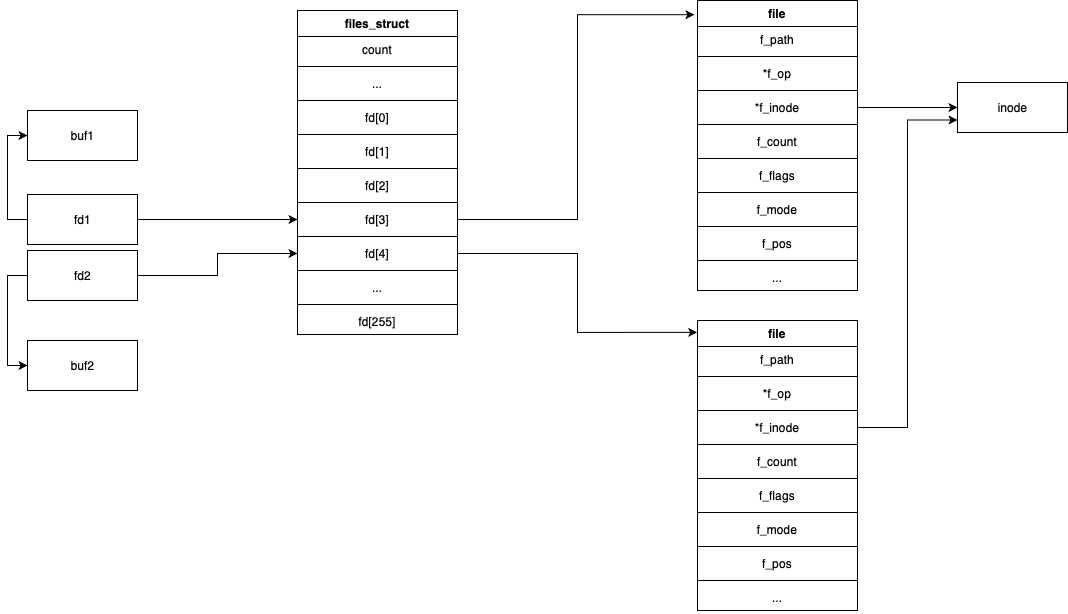
\includegraphics[scale=0.45]{pics/proc3.png}
		
			Рис 0.11: Связь структур для третьей программы
\end{center}

Результат работы третьей программы представлен на рисунке 0.12.

\begin{center}
		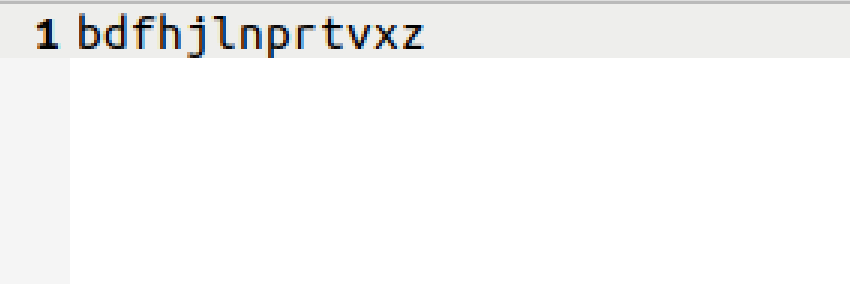
\includegraphics[scale=0.5]{pics/Res3.png}
		
			Рис 0.12: Результат работы третьей программы
\end{center}

Такой вывод объясняется порядком вызова функции fclose(). Функция fclose() отделяет указанный поток от связанного с ним файла. Если поток использовался для вывода данных, то все данные, содержащиеся в буфере, сначала записаны в файл. 

Так как сначала fclose() была вызвана для fd1, символы в буфере для fd1 были записаны в файл. Затем fclose() была вызвана для fd2, и, так как указатель смещения в файле *f\_pos разный для fd1 и fd2, символы из буфера для fd2 запишутся в файл, начиная с 0-го смещения. Тем самым, произойдет утеря данных.

Результат работы третьей программы, если поменять местами вызовы fclose(), представлен на рисунке 0.13.

\begin{center}
		
\includegraphics[scale=0.55]{pics/Res3_1.png}
		
			Рис 0.13: Результат работы третьей программы с другим порядком fclose()
\end{center}

\subsection{Структура stat}

\begin{lstlisting}[language=C]
struct stat {
               dev_t     st_dev;         /* ID of device containing file */
               ino_t     st_ino;         /* Inode number */
               mode_t    st_mode;        /* File type and mode */
               nlink_t   st_nlink;       /* Number of hard links */
               uid_t     st_uid;         /* User ID of owner */
               gid_t     st_gid;         /* Group ID of owner */
               dev_t     st_rdev;        /* Device ID (if special file) */
               off_t     st_size;        /* Total size, in bytes */
               blksize_t st_blksize;     /* Block size for filesystem I/O */
               blkcnt_t  st_blocks;      /* Number of 512B blocks allocated */

               /* Since Linux 2.6, the kernel supports nanosecond
                  precision for the following timestamp fields.
                  For the details before Linux 2.6, see NOTES. */

               struct timespec st_atim;  /* Time of last access */
               struct timespec st_mtim;  /* Time of last modification */
               struct timespec st_ctim;  /* Time of last status change */

           #define st_atime st_atim.tv_sec      /* Backward compatibility */
           #define st_mtime st_mtim.tv_sec
           #define st_ctime st_ctim.tv_sec
           };

\end{lstlisting}

Источник: Linux manual page.

\begin{lstlisting}[language=C]
stat(const char *restrict pathname,
                struct stat *restrict statbuf);
 \end{lstlisting}               
\textbf{stat} возвращает информацию о файле pathname и заполняет буфер statbuf.

Результат работы третьей программы с использованием структуры stat представлен на рисунке 0.14.

\begin{center}
		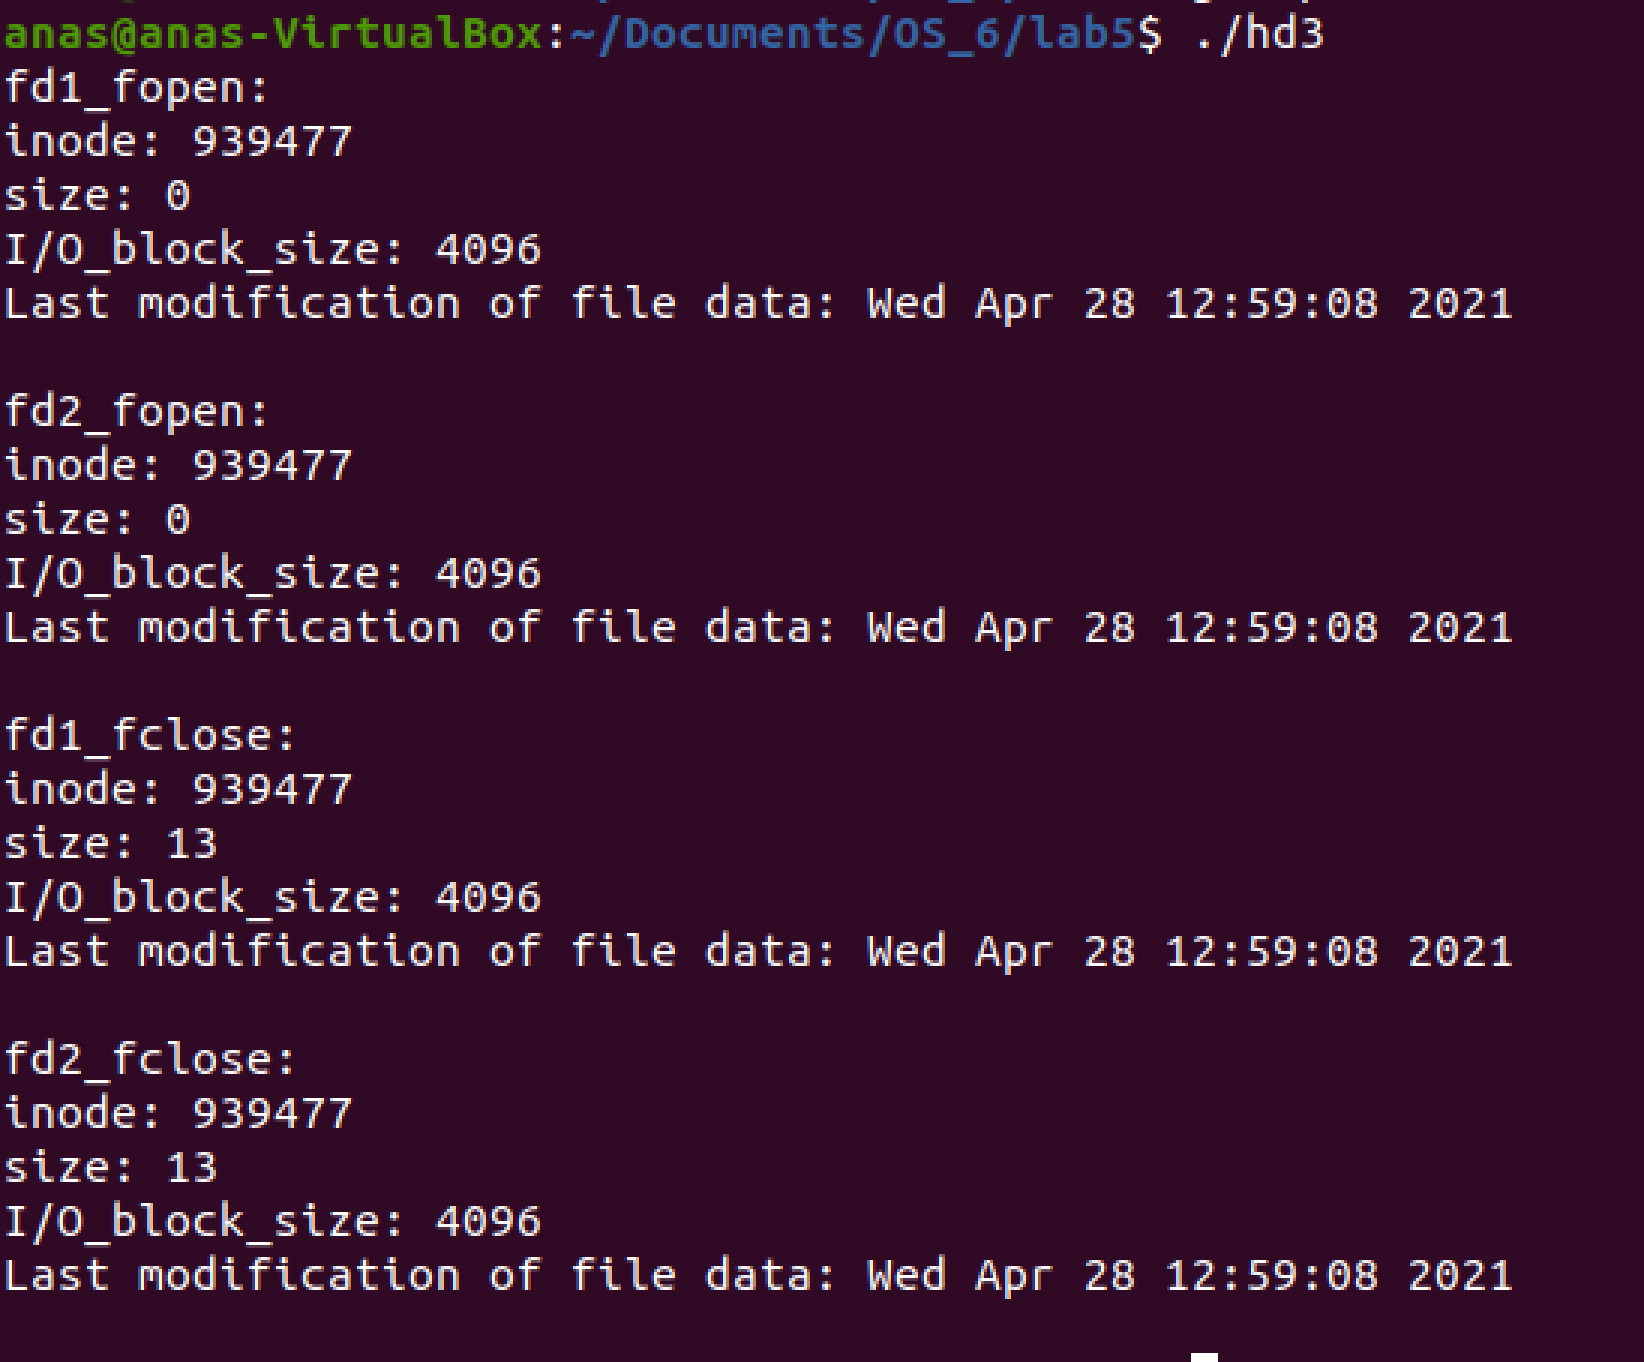
\includegraphics[scale=0.55]{pics/Stat.png}
		
			Рис 0.14: Результат работы третьей программы с использованием структуры stat 
\end{center}

\end{document}